\chapter[3D Beam-Column Element]{3D Beam-Column Element: Strength of Materials Approach}
\label{ch:beamcolumn}

\section{Stiffness matrix of a 3D beam-column element with bisymmetrical section}
{\footnotesize
\begin{equation}
  \label{eq:k3d}
  \Bmat{F_{x1}\\ F_{y1}\\ F_{z1}\\ M_{x1}\\ M_{y1}\\ M_{z1}\\ F_{x2}\\ F_{y2}\\ F_{z2}\\ M_{x2}\\ M_{y2}\\ M_{z2}}
  = E\,
  \setlength{\arraycolsep}{2.2pt}
  \left[\begin{array}{cccccc|cccccc}
    \frac{A}{L} & 0 & 0 & 0 & 0 & 0 & -\frac{A}{L} & 0 & 0 & 0 & 0 & 0\\[3pt]
    0 & \frac{12I_z}{L^3} & 0 & 0 & 0 & \frac{6I_z}{L^2} & 0 & -\frac{12I_z}{L^3} & 0 & 0 & 0 & \frac{6I_z}{L^2}\\[3pt]
    0 & 0 & \frac{12I_y}{L^3} & 0 & -\frac{6I_y}{L^2} & 0 & 0 & 0 & -\frac{12I_y}{L^3} & 0 & -\frac{6I_y}{L^2} & 0\\[3pt]
    0 & 0 & 0 & \frac{J}{2(1+\nu)L} & 0 & 0 & 0 & 0 & 0 & -\frac{J}{2(1+\nu)L} & 0 & 0\\[3pt]
    0 & 0 & -\frac{6I_y}{L^2} & 0 & \frac{4I_y}{L} & 0 & 0 & 0 & \frac{6I_y}{L^2} & 0 & \frac{2I_y}{L} & 0\\[3pt]
    0 & \frac{6I_z}{L^2} & 0 & 0 & 0 & \frac{4I_z}{L} & 0 & -\frac{6I_z}{L^2} & 0 & 0 & 0 & \frac{2I_z}{L}\\[3pt]\hline
    -\frac{A}{L} & 0 & 0 & 0 & 0 & 0 & \frac{A}{L} & 0 & 0 & 0 & 0 & 0\\[3pt]
    0 & -\frac{12I_z}{L^3} & 0 & 0 & 0 & -\frac{6I_z}{L^2} & 0 & \frac{12I_z}{L^3} & 0 & 0 & 0 & -\frac{6I_z}{L^2}\\[3pt]
    0 & 0 & -\frac{12I_y}{L^3} & 0 & \frac{6I_y}{L^2} & 0 & 0 & 0 & \frac{12I_y}{L^3} & 0 & \frac{6I_y}{L^2} & 0\\[3pt]
    0 & 0 & 0 & -\frac{J}{2(1+\nu)L} & 0 & 0 & 0 & 0 & 0 & \frac{J}{2(1+\nu)L} & 0 & 0\\[3pt]
    0 & 0 & -\frac{6I_y}{L^2} & 0 & \frac{2I_y}{L} & 0 & 0 & 0 & \frac{6I_y}{L^2} & 0 & \frac{4I_y}{L} & 0\\[3pt]
    0 & \frac{6I_z}{L^2} & 0 & 0 & 0 & \frac{2I_z}{L} & 0 & -\frac{6I_z}{L^2} & 0 & 0 & 0 & \frac{4I_z}{L}
  \end{array}\right]
  \Bmat{u_1\\ v_1\\ w_1\\ \theta_{x1}\\ \theta_{y1}\\ \theta_{z1}\\ u_2\\ v_2\\ w_2\\ \theta_{x2}\\ \theta_{y2}\\ \theta_{z2}}
\end{equation}}

The above stiffness matrix contains four parts, one arising from axial deformation, two from bending deformation, and the other from torsional deformation. We shall derive the stiffness matrices for these four parts by solving the corresponding differential equations.
\begin{fig}
  % 3D beam-column element: end forces and displacements (12 DOFs)
\begin{tikzpicture}[scale=1.0,font=\footnotesize,x={(1cm,0cm)},y={(0cm,1cm)},z={(-0.7cm,-0.5cm)}]
  \def\L{7} \def\h{0.45} \def\b{0.9}
  % member as a box
  \coordinate (n1) at (0,0,0); \coordinate (n2) at (\L,0,0);
  \draw (0,\h,\b) -- (\L,\h,\b) -- (\L,\h,-\b) -- (0,\h,-\b) -- cycle;      % top face
  \draw (0,-\h,\b) -- (\L,-\h,\b); \draw (0,-\h,-\b) -- (\L,-\h,-\b);
  \draw (0,\h,\b) -- (0,-\h,\b); \draw (0,\h,-\b) -- (0,-\h,-\b); \draw (0,-\h,\b) -- (0,-\h,-\b);
  \draw (\L,\h,\b) -- (\L,-\h,\b); \draw (\L,\h,-\b) -- (\L,-\h,-\b); \draw (\L,-\h,\b) -- (\L,-\h,-\b);
  \fill (n1) circle (0.06); \fill (n2) circle (0.06);
  \node[below right] at (n1) {1}; \node[above left] at (n2) {2};
  % --- node 1 ---
  \draw[load] (n1) -- ++(0,1.6,0) node[right] {$F_{y1},v_1$};
  \draw[load,double] (0,1.75,0) -- (0,2.9,0) node[right] {$M_{y1},\theta_{y1}$};
  \draw[load] (-1.4,0,0) -- (-0.1,0,0) node[pos=0,above] {$F_{x1},u_1$};
  \draw[load,double] (-3.2,0,0) -- (-1.7,0,0) node[pos=0,above] {$M_{x1},\theta_{x1}$};
  \draw[load] (n1) -- ++(0,0,1.5) node[below left,inner sep=1pt] {$F_{z1},w_1$};
  \draw[load,double] (0,0,1.9) -- (0,0,3.1) node[below left,inner sep=1pt] {$M_{z1},\theta_{z1}$};
  % --- node 2 ---
  \draw[load] (n2) -- ++(0,1.6,0) node[right] {$F_{y2},v_2$};
  \draw[load,double] (\L,1.75,0) -- (\L,2.9,0) node[right] {$M_{y2},\theta_{y2}$};
  \draw[load] (\L+0.1,0,0) -- (\L+1.4,0,0) node[above] {$F_{x2},u_2$};
  \draw[load,double] (\L+1.7,0,0) -- (\L+3.2,0,0) node[above] {$M_{x2},\theta_{x2}$};
  \draw[load] (n2) -- ++(0,0,1.5) node[below right,inner sep=1pt] {$F_{z2},w_2$};
  \draw[load,double] (\L,0,1.9) -- (\L,0,3.1) node[below right,inner sep=1pt] {$M_{z2},\theta_{z2}$};
  % length
  \draw[dim] (0,-2.4,0) -- (\L,-2.4,0) node[midway,fill=white,inner sep=1pt] {$L$};
  \draw (0,-2.2,0) -- (0,-2.6,0); \draw (\L,-2.2,0) -- (\L,-2.6,0);
\end{tikzpicture}

\end{fig}

\section{Axial stiffness matrix}
\begin{fig}
  % Axial bar with distributed load b(x) and a differential element
\begin{tikzpicture}[scale=1.0,font=\small]
  \begin{scope}
    \draw[thick] (0,0) rectangle (5,0.4);
    \foreach \x in {0.2,1.0,...,4.8}{\draw[->] (\x,0.75) -- (\x+0.55,0.75);}
    \node[above] at (2.5,0.85) {$b(x)$};
    \node[align=center,below] at (2.5,-0.1) {Appropriate boundary conditions\\at ends (not shown)};
  \end{scope}
  \begin{scope}[xshift=8cm]
    \draw[thick] (0,0) rectangle (1.0,0.4);
    \draw[->] (0.2,0.75) -- (0.8,0.75); \node[above] at (0.5,0.85) {$b(x)dx$};
    \draw[load] (0,0.2) -- (-0.9,0.2) node[left] {$EAu'$};
    \draw[load] (1.0,0.2) -- (1.9,0.2) node[right] {$EAu'+EAu''dx$};
    \draw[->] (-0.6,-0.4) -- (0,-0.4); \draw[->] (1.6,-0.4) -- (1.0,-0.4);
    \node[below] at (0.5,-0.25) {$dx$};
    \draw (0,-0.6) -- (0,-0.2); \draw (1,-0.6) -- (1,-0.2);
  \end{scope}
\end{tikzpicture}

\end{fig}
\begin{equation*}
  \textstyle\sum F_x = 0:\qquad EAu''\,dx + b(x)\,dx = 0
\end{equation*}
If $b(x) = 0$ then $EAu'' = 0$.
\begin{align*}
  \text{Governing equation (G.E.):}&\quad EAu''(x) = 0\quad(\text{assume } EA = \text{constant}),\ 0 < x < L\\
  \text{Boundary conditions (BCs):}&\quad u(0) = u_1\ \text{ and }\ u(L) = u_2
\end{align*}
Integrating the G.E. twice, we obtain
\begin{equation*}
  u(x) = c_1x + c_2.
\end{equation*}
Using the BCs, we obtain
\begin{equation*}
  c_2 = u_1,\qquad c_1L + c_2 = u_2.
\end{equation*}
Solving the above two equations yields
\begin{equation*}
  c_1 = (u_2-u_1)/L,\qquad c_2 = u_1.
\end{equation*}
Therefore,
\begin{equation}
  u(x) = c_1x + c_2 = u_1\Bigl(1-\frac{x}{L}\Bigr) + u_2\frac{x}{L} = N_1(x)u_1 + N_2(x)u_2
\end{equation}
where
\begin{equation}
  N_1(x) = 1-\frac{x}{L},\qquad N_2(x) = \frac{x}{L}.
\end{equation}
Finally,
\begin{align}
  F_{x1} &= -EAu'(0) = \frac{EA}{L}(u_1-u_2)\\
  F_{x2} &= EAu'(L) = \frac{EA}{L}(-u_1+u_2)
\end{align}
That is,
\begin{equation}
  \Bmat{F_{x1}\\ F_{x2}} = \frac{EA}{L}\bmat{1 & -1\\ -1 & 1}\Bmat{u_1\\ u_2}.
\end{equation}

\topic{Energy method:}
We can also derive the stiffness matrix from the strain energy. Since $u(x) = u_1(1-\frac{x}{L}) + u_2\frac{x}{L} = \NN\bs{\Delta}$, where $\NN(x) = \langle N_1, N_2\rangle$ and $\bs{\Delta} = \langle u_1, u_2\rangle^\tr$, the strain energy can be written as
\begin{equation}
  U = \frac12\int_0^L EA(u')^2\,dx = \frac12 EA\int_0^L (u')^\tr u'\,dx
    = \frac12 EA\int_0^L \bs{\Delta}^\tr\NN'^{\tr}\NN'\bs{\Delta}\,dx = \frac12\bs{\Delta}^\tr\kmat\bs{\Delta}.
\end{equation}
Therefore,
\begin{equation}
  \kmat = EA\int_0^L \NN'^{\tr}\NN'\,dx.
\end{equation}

\section{Flexural stiffness matrix for bending w.r.t.\ the \texorpdfstring{$z$}{z}-axis}
$\theta_z(x) = v'(x)$
\begin{align*}
  \text{Governing equation (G.E.):}&\quad EI_z v^{(iv)}(x) = 0\quad(\text{assume } EI_z = \text{constant}),\ 0 < x < L\\
  \text{Boundary conditions (BCs):}&\quad v(0) = v_1,\ v(L) = v_2,\ v'(0) = \theta_{z1},\ \text{and } v'(L) = \theta_{z2}.
\end{align*}
\begin{fig}
  % Bending about the z-axis: v(x) and v'(x) > 0
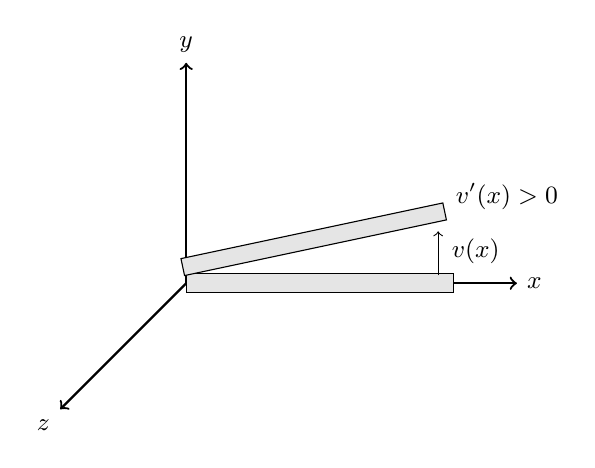
\begin{tikzpicture}[scale=1.0,font=\small]
  \draw[->,thick] (0,0) -- (4.2,0) node[right] {$x$};
  \draw[->,thick] (0,0) -- (0,2.8) node[above] {$y$};
  \draw[->,thick] (0,0) -- (-1.6,-1.6) node[below left] {$z$};
  % undeformed and deformed beam
  \draw[fill=black!10] (0,-0.12) rectangle (3.4,0.12);
  \draw[fill=black!10,rotate=12] (0,0.1) rectangle (3.4,0.32);
  \draw[->] (3.2,0.1) -- (3.2,0.66); \node[right] at (3.25,0.4) {$v(x)$};
  \node[right] at (3.3,1.1) {$v'(x)>0$};
\end{tikzpicture}

\end{fig}
Integrating the G.E. four times, we obtain
\begin{equation}
  v(x) = \frac16 c_1x^3 + \frac12 c_2x^2 + c_3x + c_4.
\end{equation}
Using the four boundary conditions, we obtain
\begin{equation}
  \bmat{0 & 0 & 0 & 1\\ L^3/6 & L^2/2 & L & 1\\ 0 & 0 & 1 & 0\\ L^2/2 & L & 1 & 0}\Bmat{c_1\\ c_2\\ c_3\\ c_4} = \Bmat{v_1\\ v_2\\ \theta_{z1}\\ \theta_{z2}}.
\end{equation}
Solving the above system, we obtain
\begin{align*}
  c_1 &= \frac{12}{L^3}(v_1-v_2) + \frac{6}{L^2}(\theta_{z1}+\theta_{z2})\\
  c_2 &= \frac{6}{L^2}(-v_1+v_2) - \frac1L(4\theta_{z1}+2\theta_{z2})\\
  c_3 &= \theta_{z1}\\
  c_4 &= v_1
\end{align*}
Therefore,
\begin{equation}
  \begin{aligned}
    v(x) &= \frac{x^3}{6}\Bigl[\frac{12}{L^3}(v_1-v_2)+\frac{6}{L^2}(\theta_{z1}+\theta_{z2})\Bigr]
          + \frac{x^2}{2}\Bigl[\frac{6}{L^2}(-v_1+v_2)-\frac1L(4\theta_{z1}+2\theta_{z2})\Bigr] + \theta_{z1}x + v_1\\
         &= N_1(x)v_1 + N_2(x)\theta_{z1} + N_3(x)v_2 + N_4(x)\theta_{z2}
  \end{aligned}
\end{equation}
where the shape functions are shown below.
\begin{fig}
  % Hermitian shape functions N1..N4 of a beam element
\begin{tikzpicture}[scale=1.0,font=\small,
  wall/.style={fill=black!50,draw=none},
  declare function={N1(\x)=1-3*\x^2+2*\x^3; N2(\x)=\x*(1-\x)^2; N3(\x)=3*\x^2-2*\x^3; N4(\x)=\x^3-\x^2;}]
  \def\L{5.5}
  % ---- N1 ----
  \begin{scope}
    \node[anchor=west] at (-0.2,1.6) {$N_1(x) = 1-3\bigl(\tfrac{x}{L}\bigr)^2+2\bigl(\tfrac{x}{L}\bigr)^3$};
    \draw[dashed] (0,0) -- (\L,0);
    \fill[wall] (-0.2,-0.25) rectangle (0,0.25); \fill[wall] (-0.2,0.75) rectangle (0,1.25);
    \fill[wall] (\L,-0.25) rectangle (\L+0.2,0.25);
    \draw[member,domain=0:1,samples=60,variable=\t] plot ({\t*\L},{N1(\t)});
    \draw[dim] (-0.5,0) -- (-0.5,1) node[midway,left] {1};
  \end{scope}
  % ---- N2 ----
  \begin{scope}[yshift=-3.2cm]
    \node[anchor=west] at (-0.2,1.6) {$N_2(x) = x\bigl(1-\tfrac{x}{L}\bigr)^2$};
    \draw[dashed] (0,0) -- (\L,0);
    \pic at (0,0) {pin}; \fill[wall] (\L,-0.25) rectangle (\L+0.2,0.25);
    \draw[member,domain=0:1,samples=60,variable=\t] plot ({\t*\L},{N2(\t)*\L});
    \draw[thin] (0,0) -- (1.3,1.3);
    \draw[->] (1.0,0) arc (0:45:1.0); \node at (1.2,0.35) {1};
  \end{scope}
  % ---- N3 ----
  \begin{scope}[yshift=-6.4cm]
    \node[anchor=west] at (-0.2,1.6) {$N_3(x) = 3\bigl(\tfrac{x}{L}\bigr)^2-2\bigl(\tfrac{x}{L}\bigr)^3$};
    \draw[dashed] (0,0) -- (\L,0);
    \fill[wall] (-0.2,-0.25) rectangle (0,0.25);
    \fill[wall] (\L,-0.25) rectangle (\L+0.2,0.25); \fill[wall] (\L,0.75) rectangle (\L+0.2,1.25);
    \draw[member,domain=0:1,samples=60,variable=\t] plot ({\t*\L},{N3(\t)});
    \draw[dim] (\L+0.5,0) -- (\L+0.5,1) node[midway,right] {1};
  \end{scope}
  % ---- N4 ----
  \begin{scope}[yshift=-9.4cm]
    \node[anchor=west] at (-0.2,1.4) {$N_4(x) = \dfrac{x^3}{L^2}-\dfrac{x^2}{L}$};
    \draw[dashed] (0,0) -- (\L,0);
    \fill[wall] (-0.2,-0.25) rectangle (0,0.25); \pic at (\L,0) {pin};
    \draw[member,domain=0:1,samples=60,variable=\t] plot ({\t*\L},{N4(\t)*\L});
    \draw[thin] (\L,0) -- (\L-1.3,-1.3);
    \draw[->] (\L-1.0,0) arc (180:225:1.0); \node at (\L-1.25,-0.3) {1};
  \end{scope}
\end{tikzpicture}

\end{fig}
Finally,
\begin{align}
  F_{y1} &= V_y(0) = EI_z v'''(0) = \frac{EI_z}{L}\Bigl(\frac{12}{L^2}v_1 + \frac6L\theta_{z1} - \frac{12}{L^2}v_2 + \frac6L\theta_{z2}\Bigr)\\
  M_{z1} &= -M_z(0) = -EI_z v''(0) = \frac{EI_z}{L}\Bigl(\frac6L v_1 + 4\theta_{z1} - \frac6L v_2 + 2\theta_{z2}\Bigr)\\
  F_{y2} &= -V_y(L) = -EI_z v'''(L) = \frac{EI_z}{L}\Bigl(-\frac{12}{L^2}v_1 - \frac6L\theta_{z1} + \frac{12}{L^2}v_2 - \frac6L\theta_{z2}\Bigr)\\
  M_{z2} &= M_z(L) = EI_z v''(L) = \frac{EI_z}{L}\Bigl(\frac6L v_1 + 2\theta_{z1} - \frac6L v_2 + 4\theta_{z2}\Bigr)
\end{align}
In matrix form,
\begin{equation}
  \Bmat{F_{y1}\\ M_{z1}\\ F_{y2}\\ M_{z2}} = \frac{EI_z}{L}
  \begin{bmatrix}
    \dfrac{12}{L^2} & \dfrac6L & -\dfrac{12}{L^2} & \dfrac6L\\[8pt]
    \dfrac6L & 4 & -\dfrac6L & 2\\[8pt]
    -\dfrac{12}{L^2} & -\dfrac6L & \dfrac{12}{L^2} & -\dfrac6L\\[8pt]
    \dfrac6L & 2 & -\dfrac6L & 4
  \end{bmatrix}
  \Bmat{v_1\\ \theta_{z1}\\ v_2\\ \theta_{z2}}
\end{equation}

\topic{Energy method:}
Knowing that $v(x) = \NN\bs{\Delta}$, where $\NN(x) = \langle N_1, N_2, N_3, N_4\rangle$ and $\bs{\Delta} = \langle v_1, \theta_{z1}, v_2, \theta_{z2}\rangle^\tr$, the strain energy is
\begin{equation}
  U = \frac12\int_0^L EI_z(v'')^2\,dx = \frac12 EI_z\int_0^L (v'')^\tr v''\,dx
    = \frac12 EI_z\int_0^L \bs{\Delta}^\tr\NN''^{\tr}\NN''\bs{\Delta}\,dx = \frac12\bs{\Delta}^\tr\kmat\bs{\Delta}.
\end{equation}
Therefore,
\begin{equation}
  \kmat = EI_z\int_0^L \NN''^{\tr}\NN''\,dx.
\end{equation}

\section{Flexural stiffness matrix for bending w.r.t.\ the \texorpdfstring{$y$}{y}-axis}
$\theta_y(x) = -w'(x)$
\begin{fig}
  % Bending about the y-axis: w(x) and w'(x) > 0
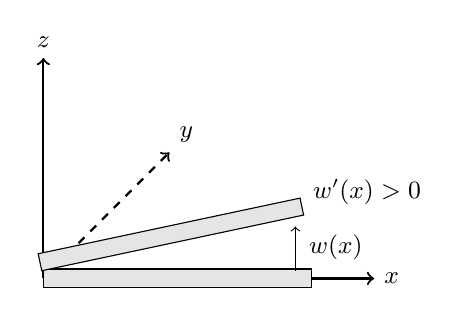
\begin{tikzpicture}[scale=1.0,font=\small]
  \draw[->,thick] (0,0) -- (4.2,0) node[right] {$x$};
  \draw[->,thick] (0,0) -- (0,2.8) node[above] {$z$};
  \draw[->,thick,dashed] (0,0) -- (1.6,1.6) node[above right] {$y$};
  \draw[fill=black!10] (0,-0.12) rectangle (3.4,0.12);
  \draw[fill=black!10,rotate=12] (0,0.1) rectangle (3.4,0.32);
  \draw[->] (3.2,0.1) -- (3.2,0.66); \node[right] at (3.25,0.4) {$w(x)$};
  \node[right] at (3.3,1.1) {$w'(x)>0$};
\end{tikzpicture}

\end{fig}
The stiffness matrix for bending w.r.t.\ the $y$-axis can be derived in a way similar to that for the $z$-axis bending, but it is noted that $w'(x) = -\theta_y(x)$; the result is
\begin{equation}
  \Bmat{F_{z1}\\ M_{y1}\\ F_{z2}\\ M_{y2}} = \frac{EI_y}{L}
  \begin{bmatrix}
    \dfrac{12}{L^2} & -\dfrac6L & -\dfrac{12}{L^2} & -\dfrac6L\\[8pt]
    -\dfrac6L & 4 & \dfrac6L & 2\\[8pt]
    -\dfrac{12}{L^2} & \dfrac6L & \dfrac{12}{L^2} & \dfrac6L\\[8pt]
    -\dfrac6L & 2 & \dfrac6L & 4
  \end{bmatrix}
  \Bmat{w_1\\ \theta_{y1}\\ w_2\\ \theta_{y2}}
\end{equation}
It shall be noted that the shape functions $N_1(x)$ and $N_3(x)$ for the $y$-axis bending are the same as those for the $z$-axis bending. However, $N_2(x)$ and $N_4(x)$ have a sign difference. Therefore, the corresponding stiffness matrices are also slightly different.

\section{Torsional stiffness matrix}
The torsional stiffness matrix can be derived in a way similar to that used in deriving the axial stiffness matrix; the result is:
\begin{equation}
  \Bmat{M_{x1}\\ M_{x2}} = \frac{GJ}{L}\bmat{1 & -1\\ -1 & 1}\Bmat{\theta_{x1}\\ \theta_{x2}}.
\end{equation}
The table below is adopted from I.~A.~Macleod (1990), \emph{Analytical Modelling of Structural Systems}, Ellis Horwood Limited, page 203. Note that the torsion constant is written as $J$ in this course.

\begin{table}[H]
  \centering\small
  \caption{St Venant torsion constant $C$ (after Macleod, 1990, Table A3).}
  \renewcommand{\arraystretch}{1.2}
  \begin{tabular}{@{}>{\raggedright\arraybackslash}p{0.3\textwidth}>{\raggedright\arraybackslash}p{0.64\textwidth}@{}}
    \toprule
    Shape & $C$\\
    \midrule
    Circular section & $C =$ second polar moment of area $= \pi R^4/2$\\[4pt]
    Closed thin-walled section & $C = \dfrac{4A_0^2}{\displaystyle\oint\frac{ds}{t}}$\rule[-22pt]{0pt}{44pt}\newline
      $A_0$ is the area enclosed by a line through the mid-thickness.\newline
      The integral is carried out along the perimeter.\\[6pt]
    Narrow rectangle, $\dfrac bt > 5$ & \begin{tikzpicture}[scale=1.0,font=\scriptsize,baseline=(current bounding box.center)]
  \draw (0,0) rectangle (2.4,0.35); \node[above] at (1.2,0.35) {$b$}; \node[right] at (2.4,0.17) {$t$};
\end{tikzpicture}
\qquad $C = \dfrac13 bt^3$\rule[-10pt]{0pt}{26pt}\\[6pt]
    Open section composed of narrow rectangles & $C = \sum\dfrac13 bt^3$\rule[-10pt]{0pt}{24pt}\newline
      $b$ is the larger dimension of a rectangle\newline
      $t$ is the width of the rectangle\newline
      The summation is over all rectangles\\[6pt]
    Closed rectangular thick-walled section & See Marshall (1970)\\[6pt]
    Solid rectangle & \begin{tikzpicture}[scale=1.0,font=\scriptsize,baseline=(current bounding box.center)]
  \draw (0,0) rectangle (2.4,0.7); \node[below] at (1.2,0) {$b$}; \node[right] at (2.4,0.35) {$t$};
\end{tikzpicture}
\rule[-14pt]{0pt}{20pt}\newline
      $C = bt^3\Bigl[\dfrac13 - 0.21\dfrac tb\Bigl(1-\dfrac{t^4}{12b^4}\Bigr)\Bigr]$\rule[-12pt]{0pt}{30pt}\\[6pt]
    Solid square & \begin{tikzpicture}[scale=1.0,font=\scriptsize,baseline=(current bounding box.center)]
  \draw (0,0) rectangle (0.9,0.9); \node[above] at (0.45,0.9) {$b$}; \node[left] at (0,0.45) {$b$};
\end{tikzpicture}
\qquad $C = 0.1406\,b^4$\rule[-14pt]{0pt}{30pt}\\
    \bottomrule
  \end{tabular}
\end{table}
